\begin{tikzpicture}	
	\draw[->, very thick, red] (22:8cm) arc[radius=1, start angle=140, end angle=40] node[above, red] at (8.3, 3.3) {$w = \dfrac{1}{\overline{z}}$};
	
	\begin{tikzpicture}
	\begin{axis}[
		axis lines=middle,
		axis equal,
		xmin=-1.1,
		xmax=1.1,
		ymin=-1.1,
		ymax=1.1,
		xlabel=$z_1$,
		ylabel=$z_2$,
	]	
		\addplot [domain=-180:180, samples=100, color=yellow, ultra thick] ({cos(x)}, {sin(x)});
		\addplot [domain=-180:180, samples=100, color=white!50!orange, ultra thick] ({5/6*cos(x)}, {5/6*sin(x)});
		\addplot [domain=-180:180, samples=100, color=white!25!orange, ultra thick] ({4/6*cos(x)}, {4/6*sin(x)});
		\addplot [domain=-180:180, samples=100, color=white!50!red, ultra thick] ({3/6*cos(x)}, {3/6*sin(x)});
		\addplot [domain=-180:180, samples=100, color=white!25!red, ultra thick] ({2/6*cos(x)}, {2/6*sin(x)});
		\addplot [domain=-180:180, samples=100, color=red, ultra thick] ({1/6*cos(x)}, {1/6*sin(x)});
		
		\addplot[-, blue, ultra thick] coordinates {(0, 0) (-1.1, 0)};
		\addplot[-, white!40!blue, ultra thick] coordinates {(0, 0) ({1.1*cos(150)}, {1.1*sin(150)})};
		\addplot[-, white!60!blue, ultra thick] coordinates {(0, 0) ({1.1*cos(120)}, {1.1*sin(120)})};
		\addplot[-, white!80!blue, ultra thick] coordinates {(0, 0) ({1.1*cos(90)}, {1.1*sin(90)})};
		\addplot[-, white!60!cyan, ultra thick] coordinates {(0, 0) ({1.1*cos(60)}, {1.1*sin(60)})};
		\addplot[-, white!80!cyan, ultra thick] coordinates {(0, 0) ({1.1*cos(30)}, {1.1*sin(30)})};
		
		\addplot[-, purple, ultra thick] coordinates {(0, 0) (1.1, 0)};
		\addplot[-, cyan, ultra thick, dashed] coordinates {(0, 0) (1.1, 0)};
		
		\addplot[-, white!40!purple, ultra thick] coordinates {(0, 0) ({1.1*cos(-30)}, {1.1*sin(-30)})};
		\addplot[-, white!60!purple, ultra thick] coordinates {(0, 0) ({1.1*cos(-60)}, {1.1*sin(-60)})};
		\addplot[-, white!80!purple, ultra thick] coordinates {(0, 0) ({1.1*cos(-90)}, {1.1*sin(-90)})};
		\addplot[-, white!80!blue, ultra thick] coordinates {(0, 0) ({1.1*cos(-120)}, {1.1*sin(-120)})};
		\addplot[-, white!60!blue, ultra thick] coordinates {(0, 0) ({1.1*cos(-150)}, {1.1*sin(-150)})};
	\end{axis}
\end{tikzpicture}\hspace{2.7cm}%
	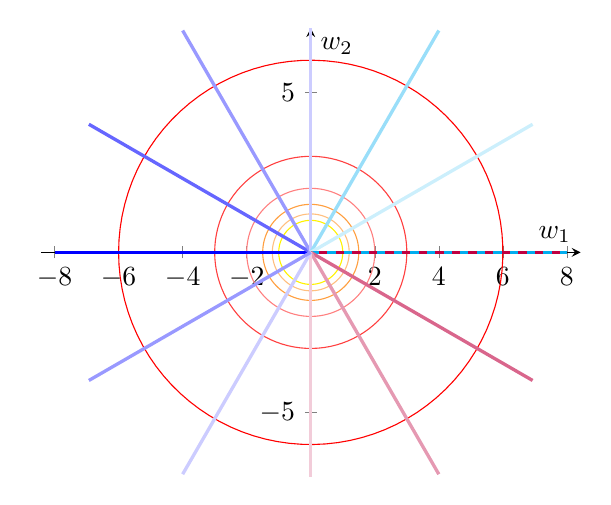
\begin{tikzpicture}
	\begin{axis}[
		axis lines=middle,
		axis equal,
		xmin=-7,
		xmax=7,
		ymin=-7,
		ymax=7,
		xlabel=$w_1$,
		ylabel=$w_2$,
	]	
		\addplot [domain=-180:180, samples=100, color=yellow] ({cos(x)/(cos(x)^2 + sin(x)^2}, {sin(x)/(cos(x)^2 + sin(x)^2});
		\addplot [domain=-180:180, samples=100, color=white!50!orange] ({(5/6*cos(x))/((5/6*cos(x))^2 + (5/6*sin(x))^2)}, {(5/6*sin(x))/((5/6*cos(x))^2 + (5/6*sin(x))^2)});
		\addplot [domain=-180:180, samples=100, color=white!25!orange] ({(4/6*cos(x))/((4/6*cos(x))^2 + (4/6*sin(x))^2)}, {(4/6*sin(x))/((4/6*cos(x))^2 + (4/6*sin(x))^2)});
		\addplot [domain=-180:180, samples=100, color=white!50!red] ({(3/6*cos(x))/((3/6*cos(x))^2 + (3/6*sin(x))^2)}, {(3/6*sin(x))/((3/6*cos(x))^2 + (3/6*sin(x))^2)});
		\addplot [domain=-180:180, samples=100, color=white!25!red] ({(2/6*cos(x))/((2/6*cos(x))^2 + (2/6*sin(x))^2)}, {(2/6*sin(x))/((2/6*cos(x))^2 + (2/6*sin(x))^2)});
		\addplot [domain=-180:180, samples=100, color=red] ({(1/6*cos(x))/((1/6*cos(x))^2 + (1/6*sin(x))^2)}, {(1/6*sin(x))/((1/6*cos(x))^2 + (1/6*sin(x))^2)});
		
		\addplot[-, blue, very thick] coordinates {(0, 0) (-8, 0)};
		\addplot[-, white!40!blue, very thick] coordinates {(0, 0) ({8*cos(150)}, {8*sin(150)})};
		\addplot[-, white!60!blue, very thick] coordinates {(0, 0) ({8*cos(120)}, {8*sin(120)})};
		\addplot[-, white!80!blue, very thick] coordinates {(0, 0) ({8*cos(90)}, {8*sin(90)})};
		\addplot[-, white!60!cyan, very thick] coordinates {(0, 0) ({8*cos(60)}, {8*sin(60)})};
		\addplot[-, white!80!cyan, very thick] coordinates {(0, 0) ({8*cos(30)}, {8*sin(30)})};
		
		\addplot[-, purple, very thick] coordinates {(0, 0) (8, 0)};
		\addplot[-, cyan, very thick, dashed] coordinates {(0, 0) (8, 0)};
		
		\addplot[-, white!40!purple, very thick] coordinates {(0, 0) ({8*cos(-30)}, {8*sin(-30)})};
		\addplot[-, white!60!purple, very thick] coordinates {(0, 0) ({8*cos(-60)}, {8*sin(-60)})};
		\addplot[-, white!80!purple, very thick] coordinates {(0, 0) ({8*cos(-90)}, {8*sin(-90)})};
		\addplot[-, white!80!blue, very thick] coordinates {(0, 0) ({8*cos(-120)}, {8*sin(-120)})};
		\addplot[-, white!60!blue, very thick] coordinates {(0, 0) ({8*cos(-150)}, {8*sin(-150)})};
	\end{axis}
\end{tikzpicture}
\end{tikzpicture}